
%(BEGIN_QUESTION)
% Copyright 2015, Tony R. Kuphaldt, released under the Creative Commons Attribution License (v 1.0)
% This means you may do almost anything with this work of mine, so long as you give me proper credit

Beregn strømmen gjennom $R_1$ i denne serie-parallell-kretsen, samt spenningen mellom punktene D og F.  Du trenger ikke angi strømretning eller spenningspolaritet.  Anta at alle motstandene er 1 k$\Omega$:

$$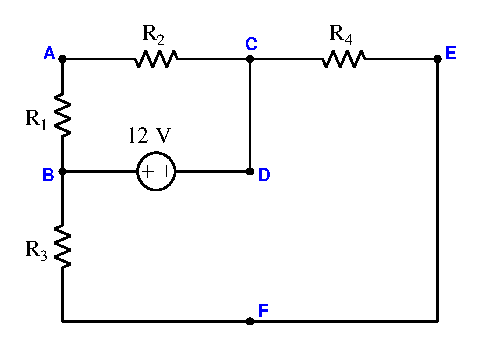
\includegraphics[width=15.5cm]{i00238x01.eps}$$

$I_{R1}$ = 

\vskip 10pt

$V_{DF}$ = 

\vskip 10pt

\underbar{file i00238}
%(END_QUESTION)





%(BEGIN_ANSWER)

$I_{R1}$ = 6 mA

\vskip 10pt

$V_{DF}$ = 6 V

%(END_ANSWER)





%(BEGIN_NOTES)

{\bf This question is intended for exams only and not worksheets!}.

%(END_NOTES)
